\section{Appendix}
\label{sec:appendix}


\begin{figure*}[t]
\centering
  \begin{minipage}{0.31\textwidth}
  \centering
  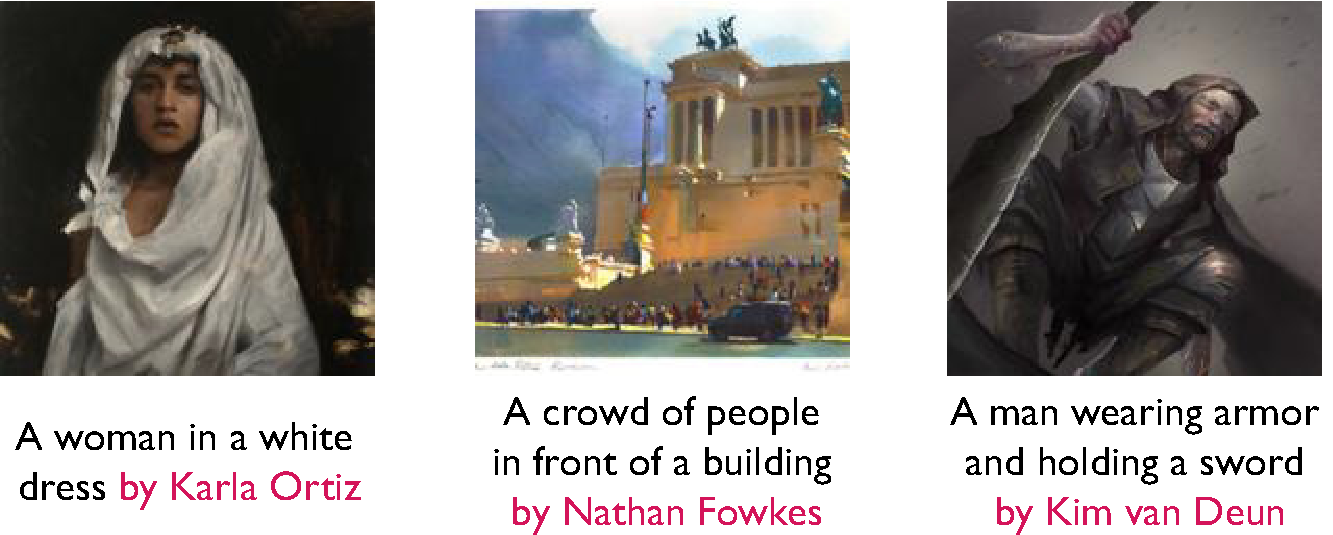
\includegraphics[width=1\columnwidth]{plots/appendix/example-image-text.pdf}
  \caption{Example data used for fine-tuning, including artwork from different
    artists and their text captions.} 
  \label{fig:data-examples}
  \end{minipage}
\hfill
  \begin{minipage}{0.31\textwidth}
  \centering
  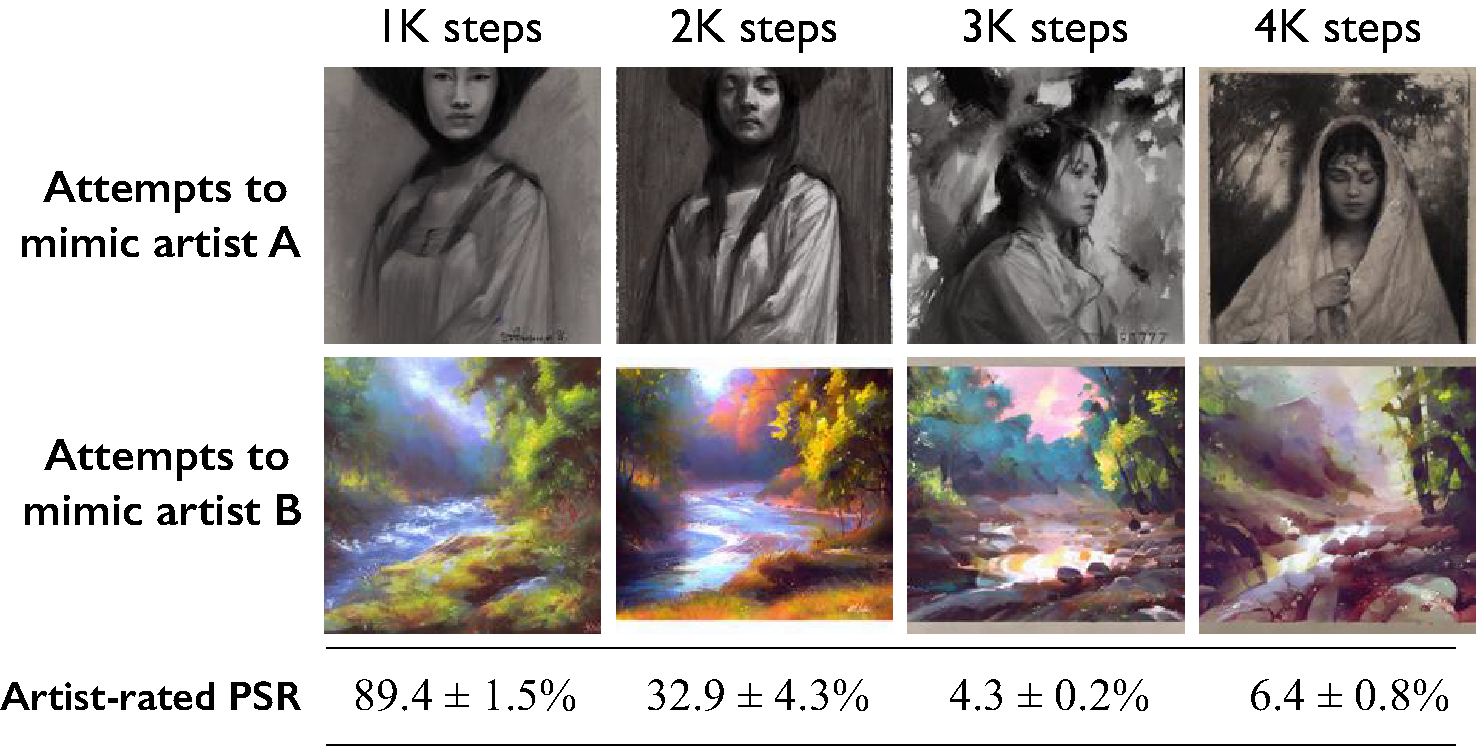
\includegraphics[width=1\columnwidth]{plots/appendix/performace-iterations.pdf}
  \caption{The success of style mimicry when the mimic fine-tunes the model for an increasing number of iterations. }
  \label{fig:success-iter}
  \end{minipage}
\hfill
  \begin{minipage}{0.31\textwidth}
  \centering
  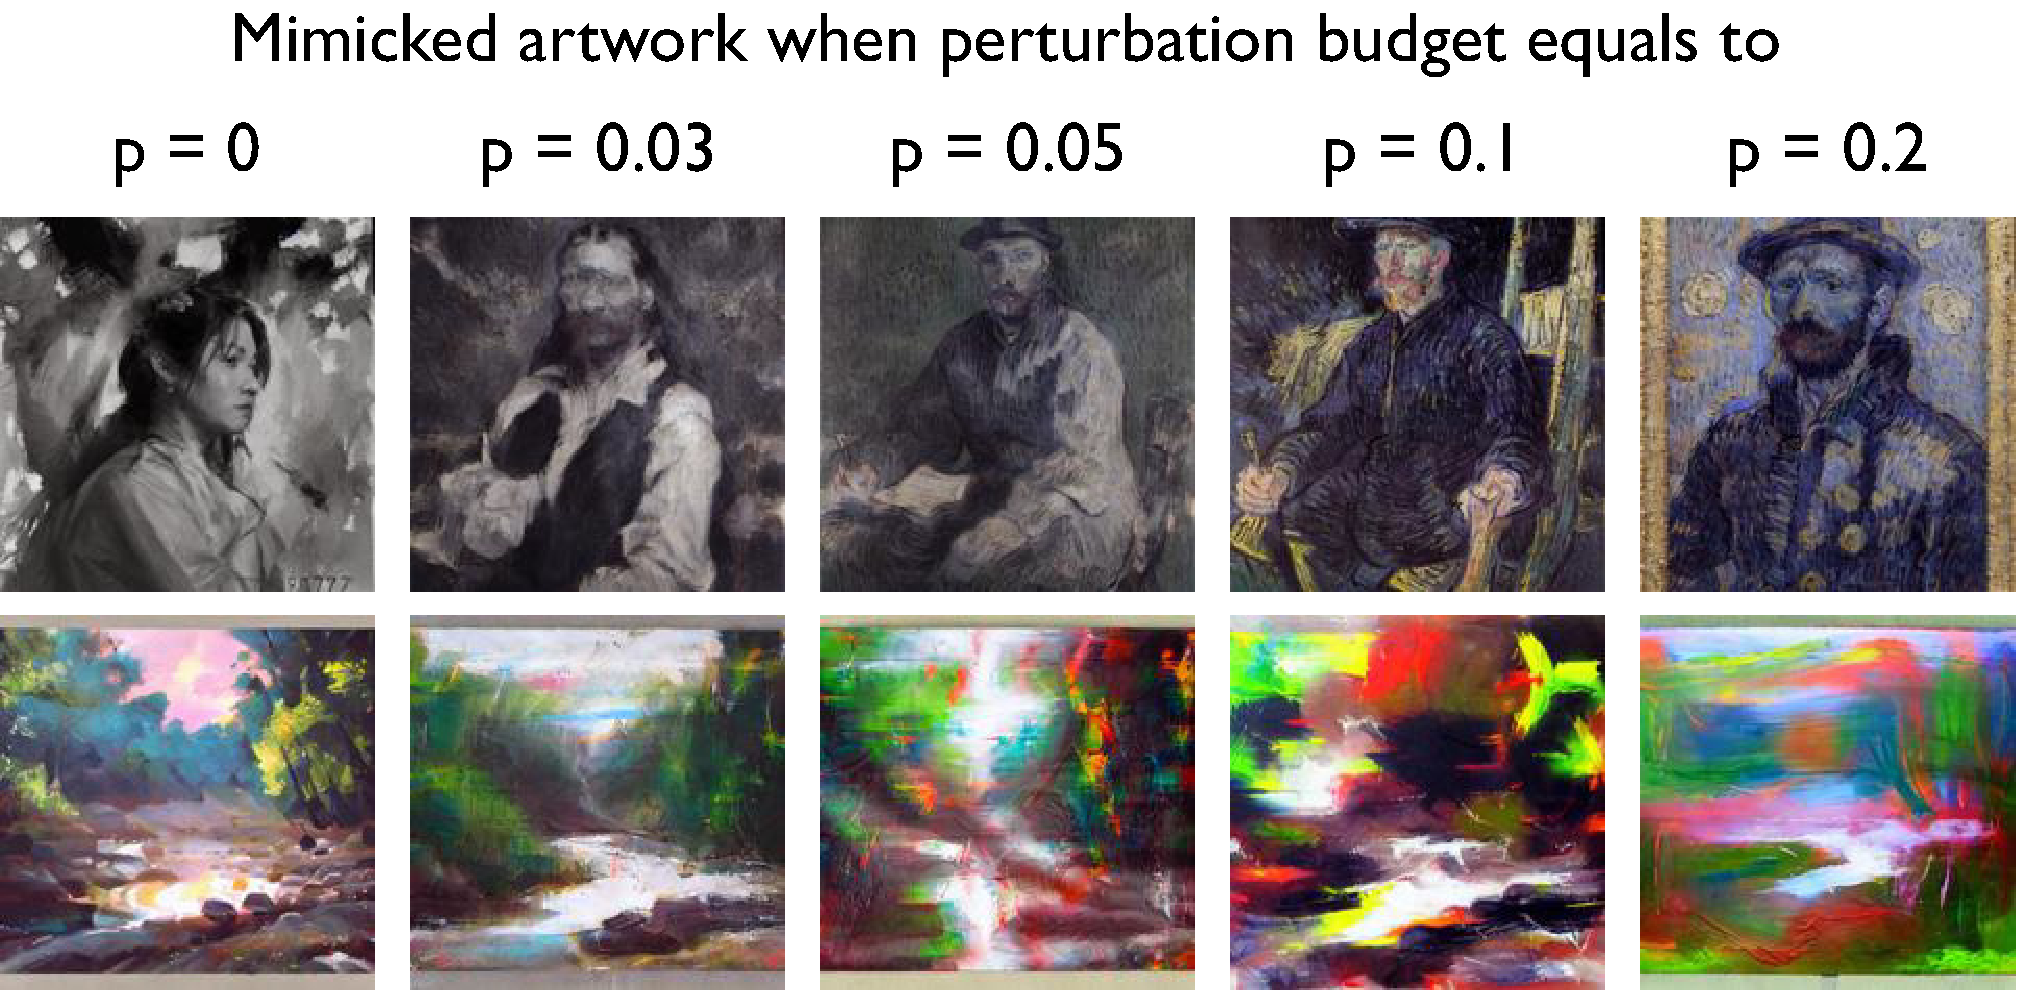
\includegraphics[width=1\columnwidth]{plots/appendix/increase-results.pdf}
  \caption{Mimicked artwork when artist uses an increasingly high
    perturbation budget to protect their original art.} 
  \label{fig:budget2results}
  \end{minipage}
  \hfill

\end{figure*}


\begin{figure*}[t]
  \begin{minipage}{0.44\textwidth}
  \centering
  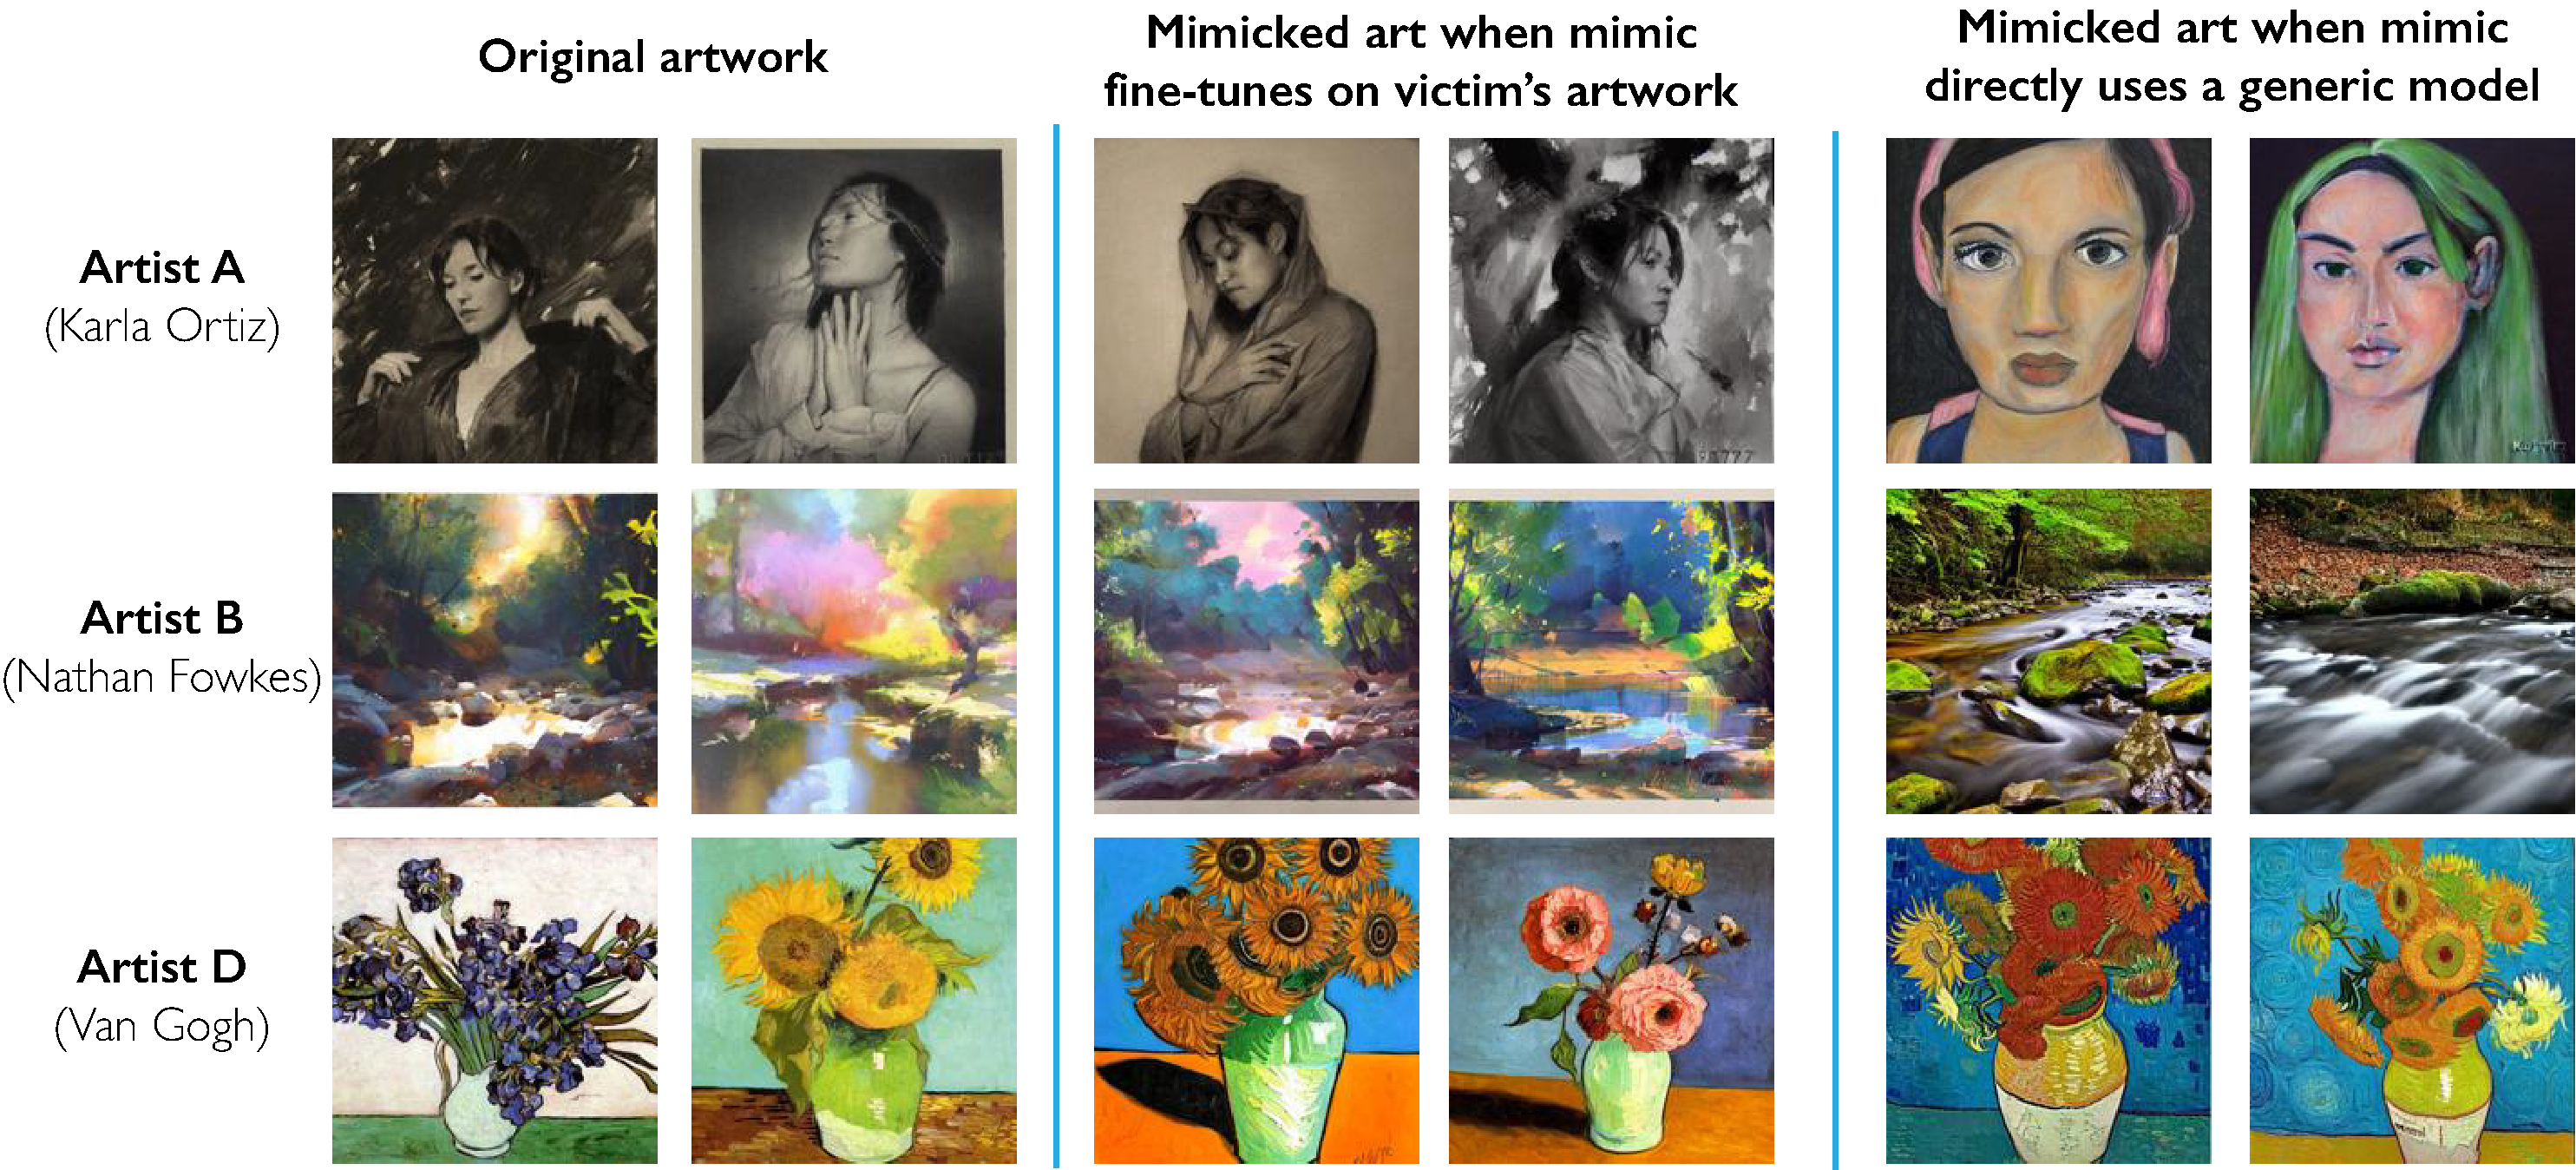
\includegraphics[width=1\columnwidth]{plots/appendix/generic-vs-finetuning.pdf}
  \vspace{-0.23in}
  \caption{Comparing performance of art mimicry directly using a generic
    model to that of mimicry on a model that has been fine-tuned on the
    victim's art pieces. \textbf{Column 1-2}: artists' original
    artwork; \textbf{column 3-4}: plagiarized artwork generated from a
    style-specific model fine-tuned on artist's art; \textbf{column
      5-6}: plagiarized artwork generated from the generic SD model using the
    artist's name as prompt.}
  \label{fig:generic-vs-finetune}
  \end{minipage}
  \hfill
\centering
  \begin{minipage}{0.48\textwidth}
  \centering
  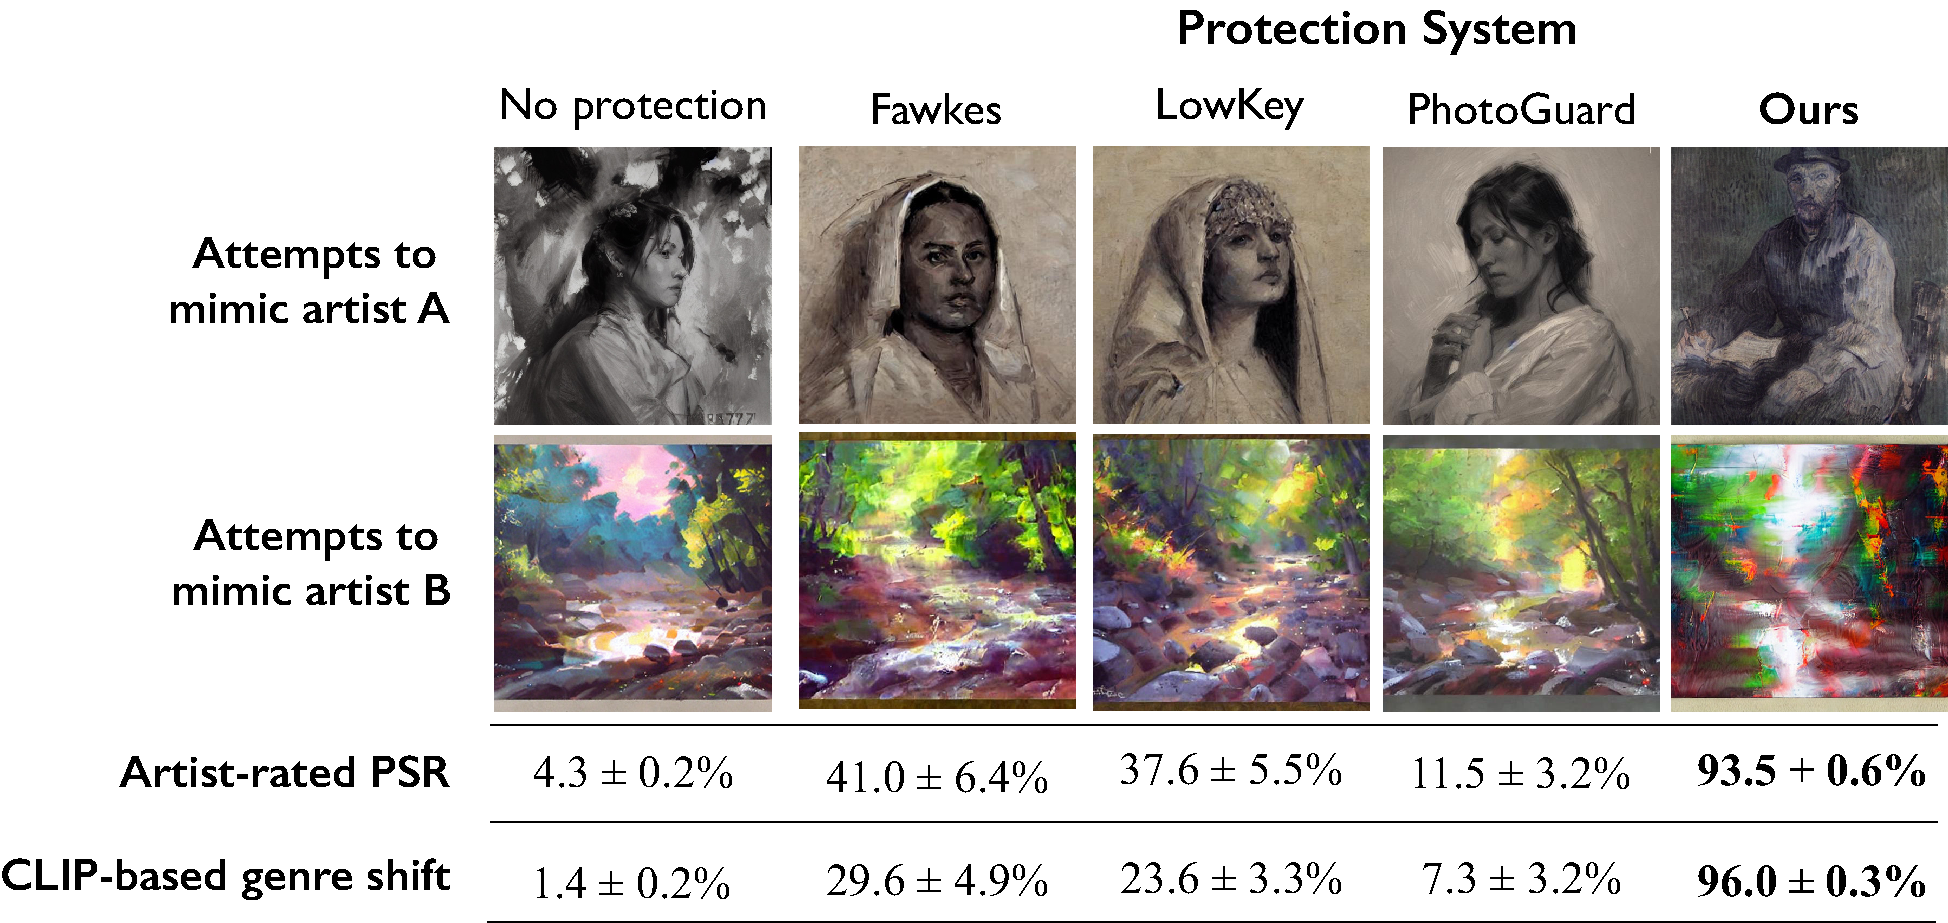
\includegraphics[width=1\columnwidth]{plots/eval/comparsion.pdf}
  \vspace{-0.23in}
  \caption{Comparing protection levels provided by different cloaking
    systems, including adapted versions of Fawkes, Lowkey, and Photoguard for style
    protection. \system{} significantly outperforms these adapted alternatives.} 
  \label{fig:existing-sys}
  \end{minipage}
  \hfill
\end{figure*}

\subsection{Adapting Existing Cloaking Systems}
\label{app:prior-work}

Here, we consider whether prior image cloaking systems can be adapted to
provide protection against art style mimicry. Our results show adapting
existing cloaking systems has limited effectiveness for our goals.

\para{Adapting existing cloaking systems. } Fawkes~\cite{shan2020fawkes}
generates a cloak on user face images by optimizing the feature space
difference between the cloaked image and a target image. The target image is
simply a face image of a different person. We adapt Fawkes to anti-mimicry
protection by switching the feature extractor from facial recognition to the
same one we use for \system. For the target image used, we assume Fawkes
randomly picks an artwork from a different artist. Fawkes uses DSSIM to bound
the input perturbation. For a fair comparison, we change Fawkes perturbation
from DSSIM to LPIPS, ones used by \system.

The general design of Lowkey~\cite{cherepanova2021lowkey} is similar to
Fawkes, except Lowkey does not optimize cloak images towards a target in
feature space but simply optimizes cloaked images to be different from the
original one. We directly apply LowKey for anti-mimicry protection: Lowkey
maximizes the cloaked artwork to have a different feature representation from
the original artwork. 

Photoguard~\cite{madry-defense} works by minimizing the norm of the image
feature vector. It is equivalent to Fawkes when Fawkes selects the zero
feature vector as the target for optimization. For anti-mimicry, we adapted
Photoguard to minimize the norm of feature representation of the cloaked
artwork. 

\para{Performance comparison. } Figure~\ref{fig:existing-sys} show Fawkes,
Lowkey, and Photoguard have limited effectiveness at protection against mimicry.
Out of the three existing systems, Fawkes achieves the best
performance with $41.0\%$ artist-rated protection success rate. While we can
see small artifacts introduced by Fawkes and Lowkey, they are not sufficient
to prevent mimicry. In our tests, we use the same LPIPS perturbation level
and the same feature extractor for optimization for all cloaking systems.  

\subsection{Additional Information on Style Mimicry}
\label{app:mimicry}

\para{Impact of fine-tuning on mimicry success. }
Figure~\ref{fig:generic-vs-finetune} compares the mimicry performance when
a mimic attack fine-tunes on the victim artist's artwork or directly using a
generic model. For artists who are not household names (e.g. iconic artists like Van Gogh),
fine-tuning significantly improves mimicry performance. We generate 
images using text captions containing the artist's name, \eg ``a river by
Nathan Fowkes.''   

\para{Details on training parameters. } For stable diffusion, we follow the
same training parameters as the original paper~\cite{rombach2022high}. We use
$5 \cdot 10^{-6}$ learning rate and batch size of $32$. For a generation, we
follow the default setting using the PNDM sampler and $50$ sampling
steps. For \dalleM, we also follow the same training setup as~\cite{d-mini} with
a learning rate of $2 \cdot 10^{-5}$ and batch size $32$. To generate images,
we use the default setting with a condition scale equal to $10$. 

\para{Impact of selecting random seed. } For diffusion-based models (\eg SD),
artwork generation is controlled by a random seed (random noise input at the
beginning). Different random seeds lead to very different images, and thus
it is common practice for mimics to generate a set of artwork using
different seed and select the best artwork. A relevant question is, can a
mimic use sheer randomness to generate a plagiarized artwork that succeeds
despite Glaze protection.

We investigate the impact of random seed selection on mimicry success in the
presence of Glaze. Given a style-specific model and a given text prompt, the
mimic generates $100$ plagiarized artworks using different random
seeds. Similar to how we calculate CLIP-based genre shift, we then use the
CLIP model to identify any artwork that belongs to the same genre as the
target artist's style. The results show that $4.3\%$ of the time, the mimic is able to find
at least $1$ out of the $100$ plagiarized artwork that passed CLIP
filtering. While the filtered artwork does belong to the same genre as the
artist, we found they tend to have lower image quality. We verify this
observation in our user study, and $> 94.1\%$ human artists rated the
protection remains successful (i.e. these art pieces failed to mimick the art
style). We believe the reason that
some plagiarized artwork still shares the same genre as victim style after
protection, is that text-to-image models today are still imperfect and often
output poor-quality images in rare cases with some random seed.

\subsection{CLIP-based metric}
\label{app:clip}

We test CLIP's performance in classifying artwork into the correct art
genre. We take $27$ historical genres from WikiArt and $13$ digital art
genres~\cite{digital-styles} as the candidate labels. We collect a test
dataset consisting of $1000$ artwork from WikiArt dataset, each containing
the ground truth labels from the Wikiart dataset. Then we collect $100$
artwork for each of the $13$ digital art genres by searching the name of the
genre on ArtStation, one of the largest digital art-sharing platforms. We
evaluate CLIP performance using top-3 accuracy as many art genres are similar
to each other (\eg impressionism vs fauvism). CLIP achieves $96.4\%$ top-3
accuracy on artwork from WikiArt and $94.2\%$ for artwork from ArtStation.  


\subsection{Additional Countermeasures} 
\label{app:counter}

\para{Details on robust training. } Here, we give details on the robust
training method we used. We follow prior work~\cite{salehi2021arae} on robust
training of autoencoder models. The mimic first uses \system{} to generate a
large number of cloaked artwork using artwork from WikiArt dataset. Given the
feature extractor $\Phi$ used by mimic's text-to-image model, the mimic trains
$\Phi$ to minimize the following loss function:  

 \begin{eqnarray}
   &\min_{\Phi} ||\Phi(x_{cloaked}) - \Phi(x_{org})||_2^2
\end{eqnarray} 
\vspace{0.1in}

\noindent where $x_{cloaked}$ and $x_{org}$ is a pair of cloaked and original
artworks. This optimization effectively forces $\Phi$ to extract the same
feature representation for cloaked and original artwork. To prevent the
extractor from collapsing (\eg output zero vectors for all inputs), we
regularized the training with the standard VAE reconstruction loss and train
the decoder $D$ at the same time. Given the high discrepancy between features
of cloaked and original artwork, this training process significantly modifies
the internals of $\Phi$ as well as the feature space. Thus, the mimic needs
to fine-tune the decoder $D$ and generator $G$ on the new robust feature
space. We assume the mimic trains $\Phi$ for $K$ steps on $K$ different pairs of
cloaked/original artwork, and then fine-tunes $D$ and $G$ until convergence.  


\begin{figure*}
  \centering
  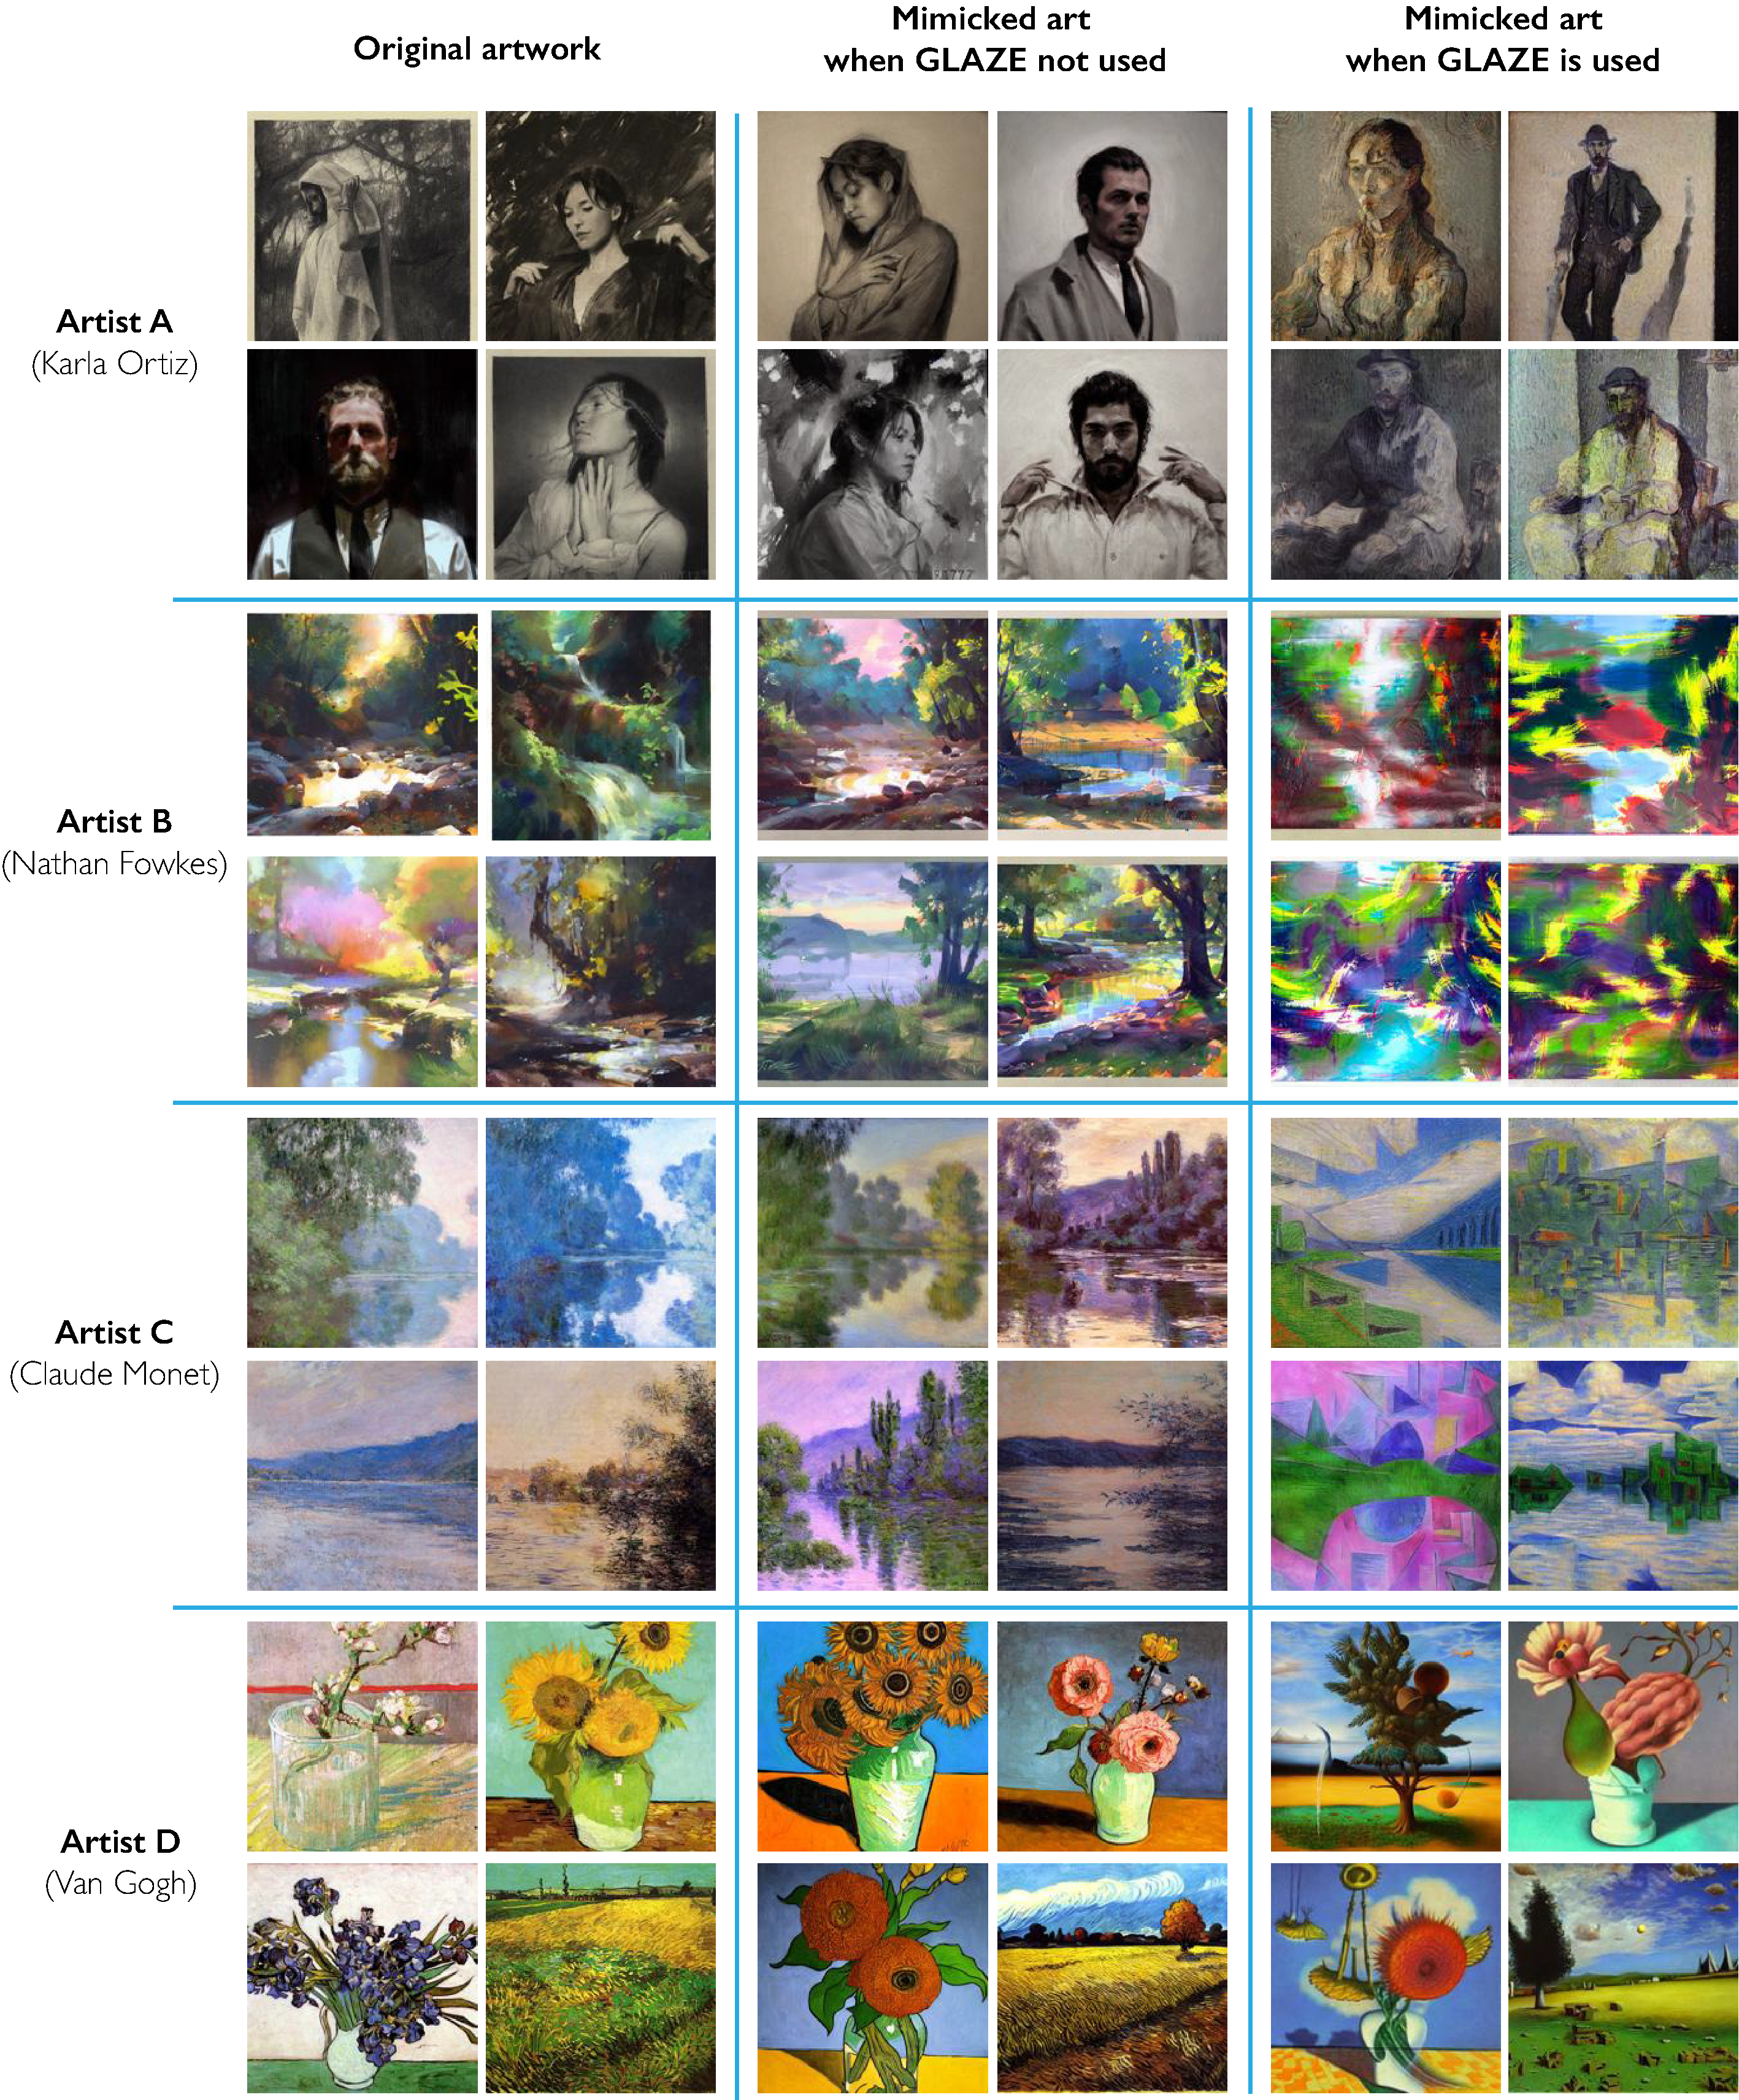
\includegraphics[width=1.0\linewidth]{plots/appendix/full-results.pdf}
  \caption{Additional example \system{} protection results for four artists. {\bf Columns 1-2}: artist's original artwork; {\bf column 3-4}: plagiarized artwork when artist does not use protection; {\bf column 5-6}: plagiarized artwork when artist uses cloaking protection with perturbation budget $p=0.05$. All mimicry attempts use SD-based models. }
  \label{fig:additional-pictures}
\end{figure*}
